\documentclass[a4paper, 12pt]{article}
\usepackage[top=2cm, bottom=2cm, left=2.5cm, right=2.5cm]{geometry}
\usepackage[utf8]{inputenc}
\usepackage[brazilian]{babel}
\usepackage{amsmath}
\usepackage{indentfirst}
\usepackage{graphicx}
\usepackage{wrapfig}
\usepackage[pdftex]{hyperref}
\graphicspath{ {imagens/} }

\begin{document}
%
\begin{titlepage} %iniciando a "capa"
	\begin{center} %centralizar o texto abaixo
		{\large Unicamp}\\[0.2cm] %0,2cm é a distância entre o texto dessa linha e o texto da próxima
		{\large [Matéria]}\\[0.2cm] % o comando \\ "manda" o texto ir para próxima linha
		{\large [Professor]}\\[3.2cm]
		{\bf \huge TÍTULO}\\[0.2cm] 
		{\bf \large Subtítulo}\\[4.9cm]
		% o comando \bf deixa o texto entre chaves em negrito. O comando \huge deixa o texto enorme
	\end{center} %término do comando centralizar
	{\large Erik Yuji Goto}\\[10cm] % o comando \large deixa o texto grande
	\begin{center}
	
		{\large Campinas}\\[0.2cm]
		{\large 2020}
	\end{center}
\end{titlepage} %término da "capa"


\tableofcontents
\newpage

\section{Conceitos Iniciais}
	\subsection{Velocidade Instântanea}
		\begin{center}
			\Large			
			$
			\vec{v(t)} = \frac{d\vec{r}}{dt}[\frac{m}{s}]			
			$
		\end{center}
	\subsection{Aceleração Instântanea}
		\begin{center}
			\Large			
			$
			\vec{a(t)}_m = \frac{d\vec{v}}{dt} = \frac{d^2\vec{r}}{d^2t} [\frac{m^2}{s}]			
			$
		\end{center}
	
	\subsection{Velocidade Angular}
		\begin{center}
			\Large			
			$
			\omega = \frac{d\theta}{dt} [\frac{rad}{s}]	
			$\\
			$
			\vec{\omega} = \dot{\theta}\hat{k}
			$			
			
		\end{center}
		
	\subsection{Aceleração Angular}
		\begin{center}
			\Large			
			$
			\alpha = \frac{d\omega}{dt} = \frac{d^2\theta}{dt^2}[\frac{rad}{s^2}]	
			$\\
			$
			\vec{\alpha} = \ddot{\omega}\hat{k}
			$			
			
		\end{center}

\section{Movimento Retilíneo da Partícula}
	\begin{figure}[h]
		\center
		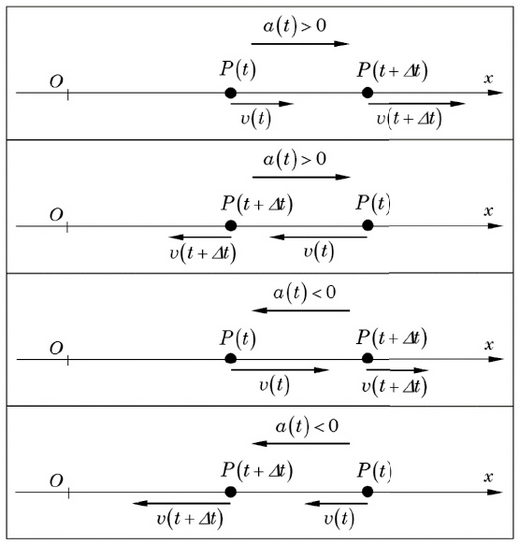
\includegraphics[scale=0.45]{imagens/mr.png} 
		\caption{Movimentos retilíneos}
	\end{figure}		
	
	\begin{enumerate}
		\item $v(t) = v_0 + at$
		\item $x(t) = x_0 + v_0t + \frac{1}{2}at^2$
		\item $v^2(x) = v_0^2+2a(x-x_0)$ - Torricelli
		\item $x(t) = x_0 + vt$
	\end{enumerate}

\section{Moviento Curvilíneo da Partícula}
	\subsection{Coordenadas Cartesianas}
		\begin{figure}[h]
			\center
			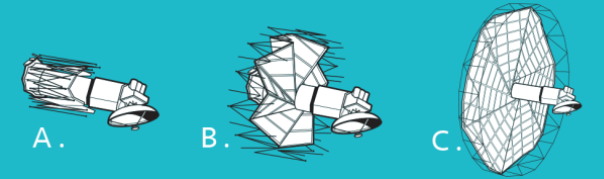
\includegraphics[scale=0.5]{imagens/c.png} 
			\caption{Cartesianas}
		\end{figure}	
		
		\begin{enumerate}
			\item $\vec{v}(t) = \dot{x}(t)\vec{i} + \dot{y}(t)\vec{j}$
			\item $\vec{a}(t) = \ddot{x}(t)\vec{i} + \ddot{y}(t)\vec{j}$
		\end{enumerate}
	\subsection{Coordenadas Normal-Tangencial}
		\begin{figure}[h]
			\center
			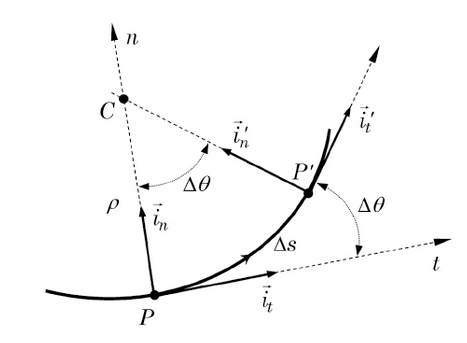
\includegraphics[scale=0.5]{imagens/t.png} 
			\caption{Normal-tangencial}
		\end{figure}		

		\begin{enumerate}
			\item $\vec{v}(t) = v(t) \hat{i}_t$
			\item $\vec{a}(t) = \frac{dv}{dt} \hat{i}_t + \frac{v^2}{\rho} \hat{i}_n$
		\end{enumerate}
	
	\subsection{Coordenadas Polares}
		\begin{figure}[h]
			\center
			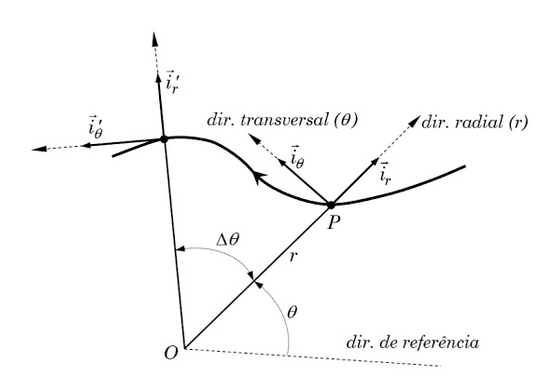
\includegraphics[scale=0.5]{imagens/pol.png} 
			\caption{Polares}
		\end{figure}	
		
		\begin{enumerate}
			\item $\vec{v}(t) = \dot{r}\vec{i}_r + r\dot{\theta} \vec{i}_{\theta}$
			\item $\vec{a}(t) = (\ddot{r} - r\dot{\theta}^2)\vec{i}_r + (r\ddot{\theta} + 2 \dot{r}\dot{\theta})\vec{i}_{\theta}$
		\end{enumerate}

\section{Movimento Circular}
	\begin{center}
		\Large
		$
		\vec{v} = (r\omega)\vec{i}_{\theta}		
		$\\
		$
		\vec{a} = (-r\omega^2)\vec{i}_r + (r\alpha)\vec{i_\theta}		
		$\\ \textit{ou}\\
		$
		\vec{v} = \vec{\omega} \times \vec{r}	
		$\\
		$
		\vec{\alpha} = \vec{\alpha} \times \vec{r} - \omega^2\vec{r}	
		$
	\end{center}

\section{Movimento Curvilíneo Espacial da Partícula}
	\subsection{Coordenadas Cartesianas}
		\begin{figure}[h]
			\center
			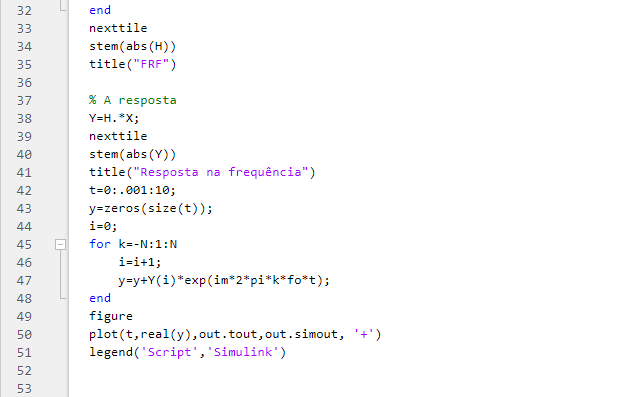
\includegraphics[scale=0.5]{imagens/cc.png} 
			\caption{Cartesianas}
		\end{figure}	
		\newpage
		\begin{figure}[h]
			\center
			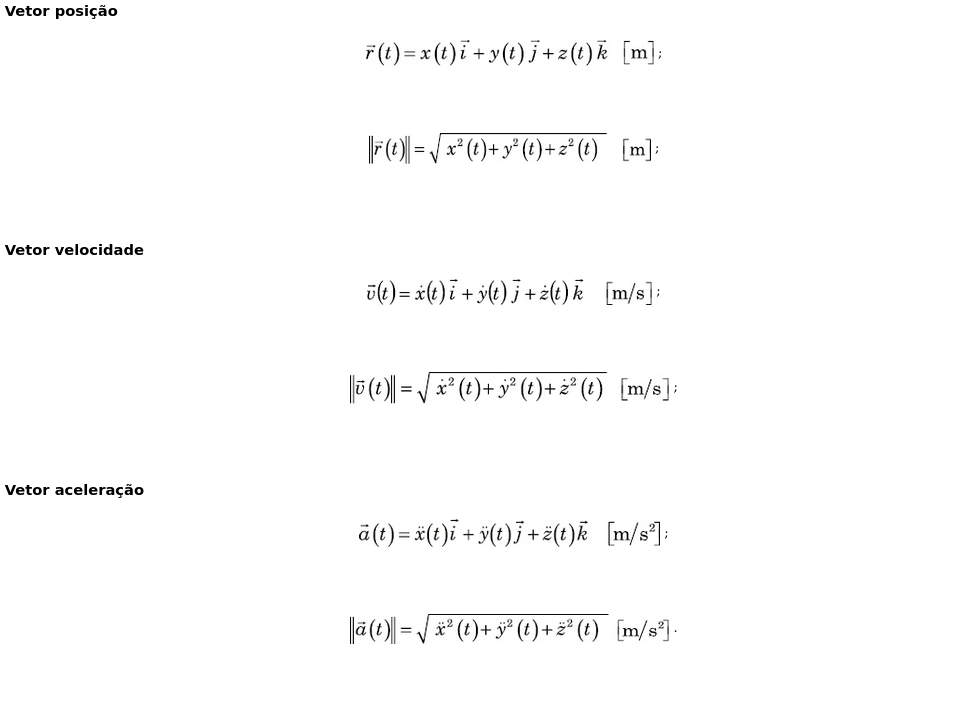
\includegraphics[scale=0.6]{imagens/ccc.png} 
			\caption{Cartesianas}
		\end{figure}

	\subsection{Coordenadas Cilíndricas}
		\begin{figure}[h]
			\center
			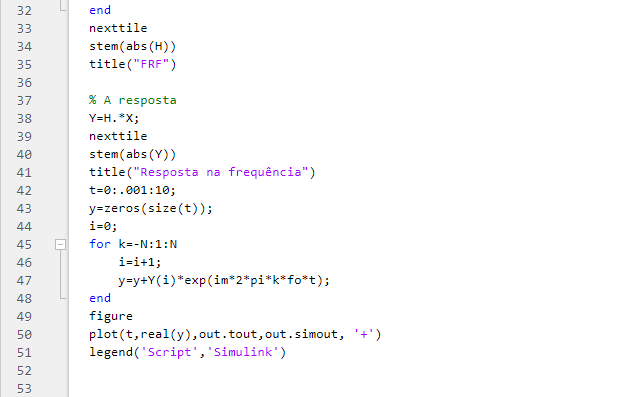
\includegraphics[scale=0.5]{imagens/cc.png} 
			\caption{Cilíndricas}
		\end{figure}	
		
		\begin{enumerate}
			\item $\vec{v} = \dot{r}\vec{i}_r + r\dot{\theta}\vec{i}_{\theta} + \dot{z}\vec{k}$
			\item $\vec{a} = (\ddot{r} - \dot{r}\dot{\theta}^2)\vec{i_r} + (r\ddot{\theta} + 2\dot{r}\dot{\theta})\vec{i_{\theta}} + \ddot{z}\vec{k}$
		\end{enumerate}
	\newpage
	\subsection{Coordenadas Esféricas}
		\begin{figure}[h]
			\center
			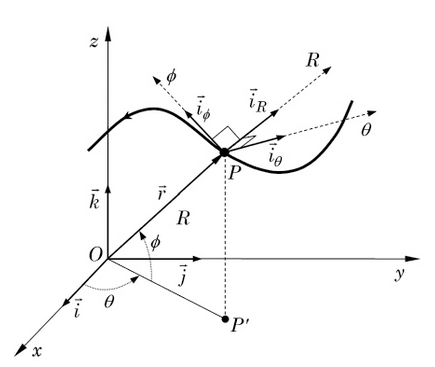
\includegraphics[scale=0.5]{imagens/e.png} 
			\caption{Esféricas}
		\end{figure}
	\begin{enumerate}
		\item $\vec{v} = \dot{R}\vec{i_R} + R\dot{\theta}cos\phi\vec{i_{\theta}} + R\dot{\phi}\vec{i}_{\phi}$
		\item 
	\end{enumerate}
		\begin{figure}[h]
			\center
			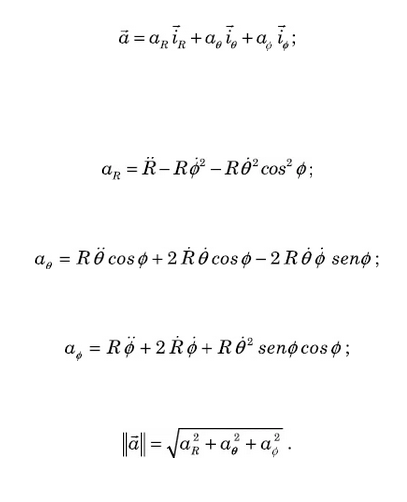
\includegraphics[scale=0.5]{imagens/ee.png} 
		\end{figure}	

\section{Transformações de Coordenadas}
\newpage

\section{Movimento Relativo}
	\subsection{Plano - Eixos de Referência em Translação}
	\begin{figure}[h]
		\center
		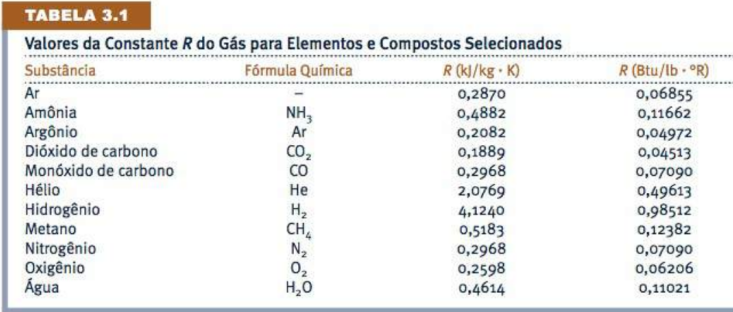
\includegraphics[scale=0.5]{imagens/r.png} 
		\caption{Cilíndricas}
	\end{figure}	

	\begin{enumerate}
		\item $\vec{r}_p = \vec{r}_A + \vec{r}_{P/A}$
		\item $\vec{v}_p = \vec{v}_A + \vec{v}_{P/A}$
		\item $\vec{a}_p = \vec{a}_A + \vec{a}_{P/A}$
	\end{enumerate}

	\subsection{Plano - Eixos de Referência em Rotação}
		\begin{figure}[h]
			\center
			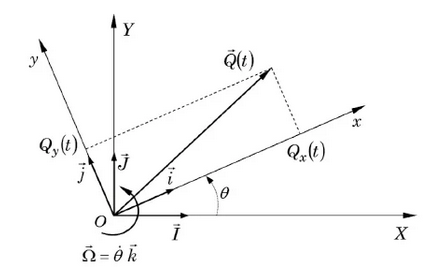
\includegraphics[scale=0.5]{imagens/rr.png} 
			\caption{Cilíndricas}
		\end{figure}	

		\begin{enumerate}
			\item $\vec{v}_p|_{OXY} = \vec{\dot{r}}_P|_{Oxy} + \vec{\Omega}\times\vec{r}_P$
			\item $\vec{a}_P|_{OXY} = \vec{\ddot{r}}_P|_{Oxy} + \vec{\dot{\Omega}}\times \vec{r}_p - \vec{\Omega}^2\vec{r}_P + 2\vec{\Omega}\times \vec{\dot{r}}_P|_{Oxy}$
		\end{enumerate}
		
	\newpage
	\subsection{Plano - Eixos de Referência em Movimento Geral}
		\begin{figure}[h]
			\center
			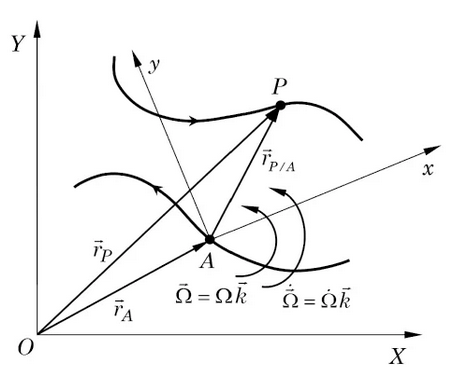
\includegraphics[scale=0.5]{imagens/ra.png} 
			\caption{Cilíndricas}
		\end{figure}	

		\begin{enumerate}
			\item $\vec{v}_P|_{OXY} = \vec{\dot{r}}_A|_{OXY} + \vec{\dot{r}}_{P/A}|_{Axy} + \vec{\Omega} \times \vec{r}_{P/A}$
			\item $\vec{a}_P|_{OXY} = \vec{\ddot{r}}_A|_{OXY} + \vec{\ddot{r}}_{P/A}|_{Axy} + \vec{\dot{\Omega}}\times \vec{r}_{P/A} - \vec{\Omega}^2\vec{r}_{P/A} + 2\vec{\Omega}\times \vec{\dot{r}}_{P/A}|_{Axy}$
		\end{enumerate}


\section{Propriedades de Inércia de Corpos Rígidos}
	\subsection{Posição do Centro de Massa de um Corpo Rígido}
		\begin{equation}
			x_G = \frac{1}{m} = \int_{vol}xdm
		\end{equation}
		\begin{equation}
			y_G = \frac{1}{m} = \int_{vol}ydm
		\end{equation}
		\begin{equation}
			z_G = \frac{1}{m} = \int_{vol}zdm
		\end{equation}
	\subsection{Posição do Centro de Massa de corpos de geometria composta}
		\begin{figure}[h]
			\center
			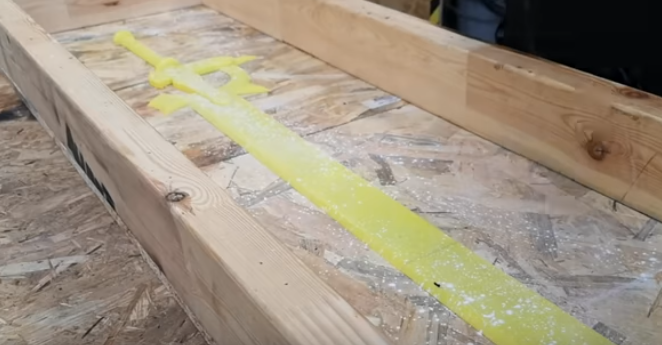
\includegraphics[scale=0.5]{imagens/a.png} 
			\caption{Corpos compostos}
		\end{figure}	
		\newpage
		\begin{equation}
			\vec{r}_G = \frac{1}{m}\sum^n_{i = 1}m_i\vec{r}_{G_i}
		\end{equation}
	\subsection{Momento de inércia de massa de um corpo rígido em relação a um eixo. Raio de giração}
		\begin{figure}[h]
			\center
			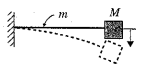
\includegraphics[scale=0.5]{imagens/a1.png} 
			\caption{Momentos de inércia}
		\end{figure}	
		O momento de inércia de massa do corpo rígido em relação ao eixo indicado é definido segundo:	
		\begin{equation}
			J_{OO'} = \int_{vol}r^2dm
		\end{equation}\\
		Nos casos em que o corpo é constituído de um material uniforme, a densidade $\rho$ é constante em todo seu volume a equação fica:
		\begin{equation}
			J_{OO'} = \rho \int_{vol}r^2dV
		\end{equation}
		O raio de giração de massa do corpo rígido em relação ao eixo OO', designado por $k_{OO'}$, é definido sob a forma:
		\begin{equation}
			k_{OO'} = \sqrt{\frac{J_{OO'}}{m}} \Leftrightarrow J_{OO'} = k^2_{OO'}m
		\end{equation}
	\newpage
	\subsection{Teorema dos Eixos Paralelos para os momentos de inércia de massa}
		\begin{figure}[h]
			\center
			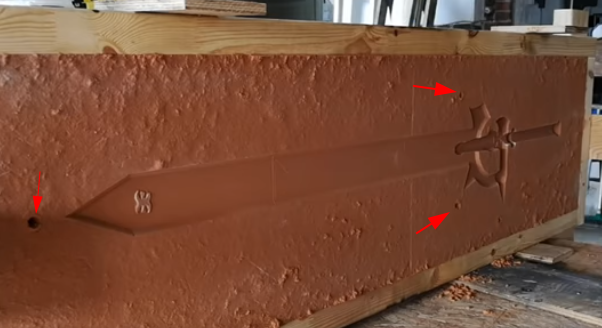
\includegraphics[scale=0.5]{imagens/a2.png} 
			\caption{Ilustração de um corpo rígido e dois eixos paralelos entre si, sendo um deles baricêntrico.}
		\end{figure}	
		Note que, um dos eixos precisa serbaricêntrico, passando pelo CG.\\
		
		Segundo o \textbf{Teorema dos Eixos Paralelos}:
			\begin{equation}
				J_{AA'} = J_{OO'} + d^2m
			\end{equation}
			\begin{equation}
				k^2_{AA'} = k^2_{OO'} + d^2
			\end{equation}
		Sendo "d" a distância perpendicular entre os dois eixos. 

	\subsection{Momentos de inércia de massa expressos em coordenadas cartesianas}
		Caso o corpo rígido seja constituído de um material uniforme, com densidade $\rho$ constante sobre seu volume, seus momentos de inércia podem ser expressas sob a forma:
		\begin{equation}
			J_x = \rho \int_{vol}(y^2 + z^2)dV
		\end{equation}
		\begin{equation}
			J_y = \rho \int_{vol}(x^2 + z^2)dV
		\end{equation}
		\begin{equation}
			J_z = \rho \int_{vol}(y^2 + x^2)dV
		\end{equation}
		\textit{No Apêndice B do Rade tem uma tabela com as propriedades do momento de inércia de alguns sólidos comuns.}
		
	\newpage
	\subsection{Momentos de inércia de corpos de geometria composta}
		\begin{figure}[h]
			\center
			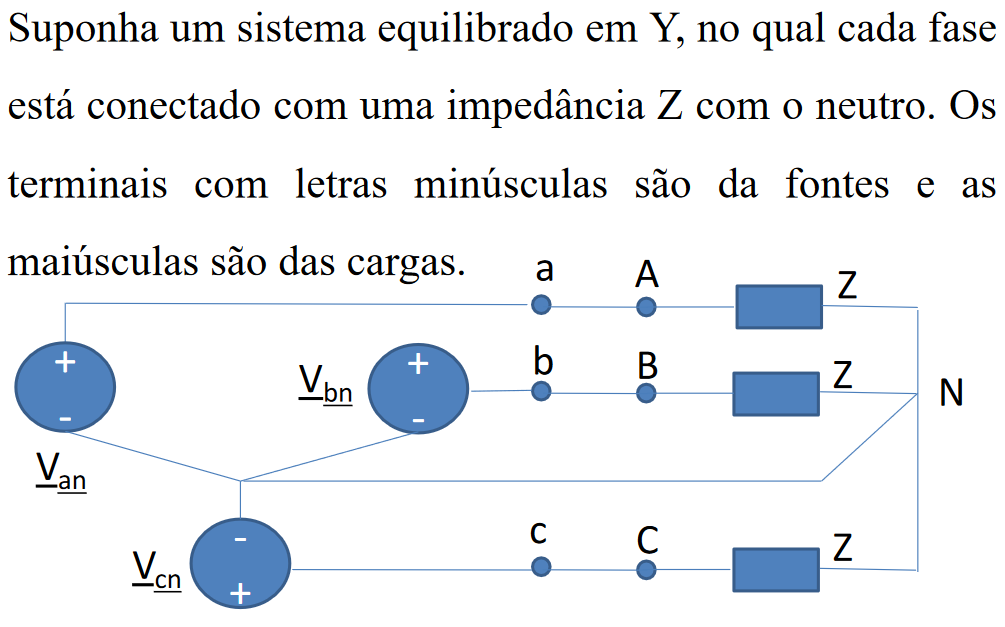
\includegraphics[scale=0.5]{imagens/a3.png} 
			\caption{Ilustração de um sólido composto pela associação de várias partes}
		\end{figure}	
		\begin{equation}
			J_x = J_x|_{P1} + J_x|_{P2} + ... + J_x|_{Pn}
		\end{equation}
		\begin{equation}
			J_y = J_y|_{P1} + J_y|_{P2} + ... + J_y|_{Pn}
		\end{equation}
		\begin{equation}
			J_z = J_z|_{P1} + J_z|_{P2} + ... + J_z|_{Pn}
		\end{equation}
	
	\subsection{Momentos de inércia de massa em relação a um eixo orientado arbitrariamente. Produtos de inércia}
		Considerando a figura, desejamos expressar o momento de inércia de massa do corpo rígido em relação ao eixo OO', orientado arbitrariamente, em função dos momentos de inércia $J_x$ , $J_y$ e $J_z$ , relativos aos eixos coordenados x, y e z. Nesta figura, o vetor $\vec{u}= u_x \vec{i}+ u_y\vec{j} + u_z\vec{k}$ é o vetor unitário na direção do eixo OO'.
		\begin{figure}[h]
			\center
			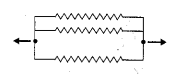
\includegraphics[scale=0.5]{imagens/a4.png} 
			\caption{Imagem que ilustra a determinação do momento de inércia de um corpo rígido em relação a um eixo orientado arbitrariamente}
		\end{figure}	
		\begin{equation}
			J_{OO'} = J_xu_x^2 + J_yu_y^2 + J_zu_z^2 - 2 P_{xy}u_xu_y- 2 P_{xz}u_xu_z - 2 P_{yz}u_yu_z
		\end{equation}
		\\
		
		Onde,
		\begin{equation}
			P_{xy} = \int_{vol} xydm
		\end{equation}
		\begin{equation}
			P_{xz} = \int_{vol} xzdm
		\end{equation}
		\begin{equation}
			P_{yz} = \int_{vol} yzdm
		\end{equation}\\
		
		Em forma matricial temos:
		\begin{equation}
			J_{OO'} = \begin{bmatrix}
			u_x & u_y & u_z 
			\end{bmatrix}\begin{bmatrix}
			J_x & -P_{xy} & -P_{xz}\\
			-P_{xy} & J_y & -P_{yz}\\
			-P_{xz} & -P_{yz} & J_z
\end{bmatrix}\begin{bmatrix}
			u_x\\ u_y \\u_z
\end{bmatrix}				
		\end{equation}

	\subsection{Teorema dos Eixos Paralelos para momentos de inércia e produtos de inércia expressos em coordenadas cartesianas}
		\begin{figure}[h]
			\center
			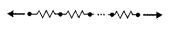
\includegraphics[scale=0.5]{imagens/a5.png} 
			\caption{Ilustração de um corpo rígido e dois sistemas de referência, sendo um deles baricêntrico}
		\end{figure}	
		Teorema dos Eixos Paralelos para os momentos de inércia expressos em coordenadas cartesianas:
		\begin{equation}
			J_x = J_{x'} + (y_G^2 + z_G^2)m
		\end{equation}
		\begin{equation}
			J_y = J_{y'} + (z_G^2 + x_G^2)m
		\end{equation}
		\begin{equation}
			J_z = J_{z'} + (y_G^2 + x_G^2)m
		\end{equation}
		Teorema dos Eixos Paralelos para os produtos de inércia em coordenadas cartesianas:
		\begin{equation}
			P_{xy} = P_{x'y'} + x_Gy_Gm
		\end{equation}
		\begin{equation}
			P_{xz} = P_{x'z'} + x_Gz_Gm
		\end{equation}
		\begin{equation}
			P_{yz} = P_{y'z'} + y_Gz_Gm
		\end{equation}

	\subsection{Eixos principais de inércia e momentos principais de inércia}
		Sempre podemos encontrar um sistema triortogonal de eixos em relação aos quais todos os \textit{produtos de inércia são nulos} simultaneamente. Neste caso, o tensor de inércia resulta ser uma matriz diagonal.\\
		
		Os eixos em relação aos quais os produtos de inércia são nulos são chamados Eixos Principais de Inércia (EPI), e os momentos de inércia em relação a estes eixos são denominados Momentos Principais de Inércia (MPI).\\
		
		Para encontrar Eixos Principais de Inérciaos e os Momentos Principais de Inércia é necessário calcular os autovetores e autovalores:
		\begin{equation}
			([J_{xyz}] - \lambda_i[I_3])\{v_i\} = \{0\}
		\end{equation}
		\begin{itemize}
			\item Os autovalores $\lambda_i$ correspondem aos valores dos três momentos principais de inércia, que designaremos por $J_{x~} , J_{y~} , J_{z~}$.
			\item Os autovetores $\{v_i\}$ são os vetores cujas componentes são os cossenos diretores dos três eixos principais de inércia, em relação ao sistema de referência Oxyz.
		\end{itemize}

\newpage
\section{Dinâmica dos Corpos rígidos}
	\subsection{Quantidade de movimento linear e quantidade de movimento angular de corpos rígidos}
	 	\begin{equation}
	 		\vec{L} = m\vec{v}_G
	 	\end{equation}
	 	\begin{equation}
	 		\vec{H}_O = \int_{vol} \vec{r} \times \vec{v}dm
	 	\end{equation}
	 	\begin{equation}
	 		\vec{H}_G = \int_{vol} \vec{r'} \times \vec{v'}dm
	 	\end{equation}
		\begin{figure}[h]
			\center
			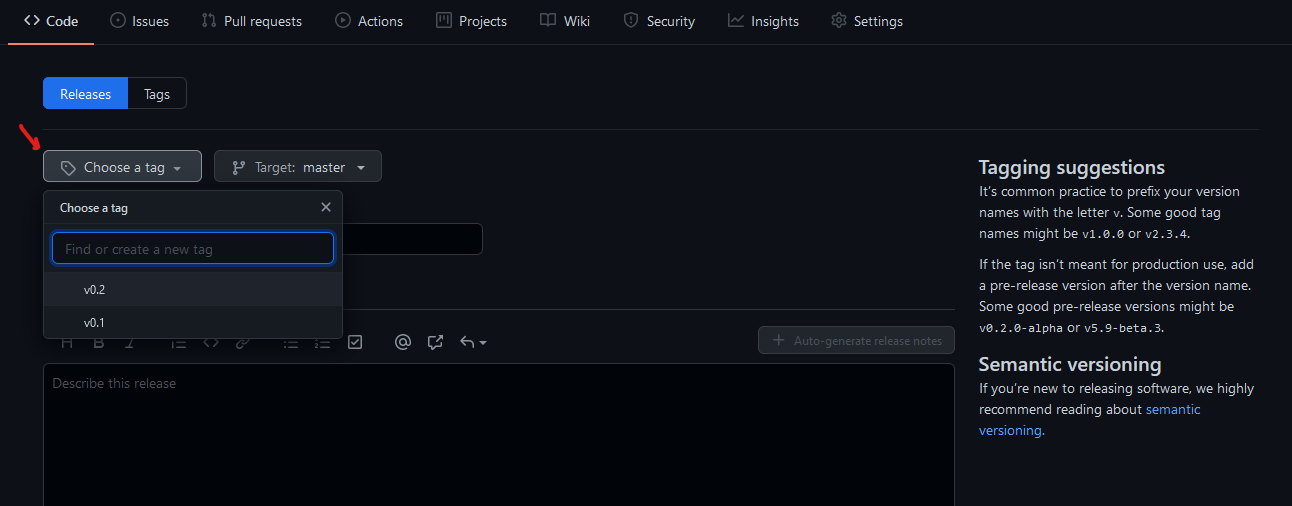
\includegraphics[scale=0.5]{imagens/a6.png} 
			\caption{Ilustração de um corpo rígido e de dois sistemas de referência}
		\end{figure}	

		Usando o tensor de inércia conseguimos calcular o momento angular:
		\begin{equation}
			\{H_G\} = [J_{Gx'y'z'}]\{\omega \}
		\end{equation}
		E, também temos:
		\begin{equation}
			\vec{H}_O = \vec{H}_G + m (\vec{r}_G \times \vec{v}_G)
		\end{equation}
	
	\subsection{Equações de Newton-Euler}
		\begin{equation}
			\sum \vec{F} = \dot{\vec{L}} = m\vec{a}_G
			\label{1}
		\end{equation}
		\begin{equation}
			\sum \vec{M}_O = \dot{\vec{H}}_O
			\label{2}
		\end{equation}
		\begin{equation}
			\sum \vec{M}_G = \dot{\vec{H}}_G
			\label{3}
		\end{equation}
		
		As equações acima, estendidas para um corpo livre, são conhecidas como Equações de Newton-Euler.
		Como as Equações \ref{2} e \ref{3} não são independentes entre si, dentre as Equações \ref{1} a \ref{3} geralmente opta-se por utilizar apenas as Equações \ref{1} e \ref{3}.
	
	\subsection{Equações de Newton-Euler para corpos rígidos em movimento de translação}
		\begin{equation}
			\sum \vec{F} = m\vec{a}_G
		\end{equation}
		\begin{equation}
			\sum \vec{M}_G = \vec{0}
		\end{equation}
		Um corpo estará em translação quando o momento resultante dos esforços externos em relação ao centro de massa for nulo. Esta condição implica que nos casos em que houver apenas forças externas aplicadas ao corpo rígido, a linha de ação da resultante destas forças deve passar pelo centro de massa do corpo.
	
	\subsection{Equações de Newton-Euler para corpos rígidos em movimento plano}
		\begin{figure}[h]
			\center
			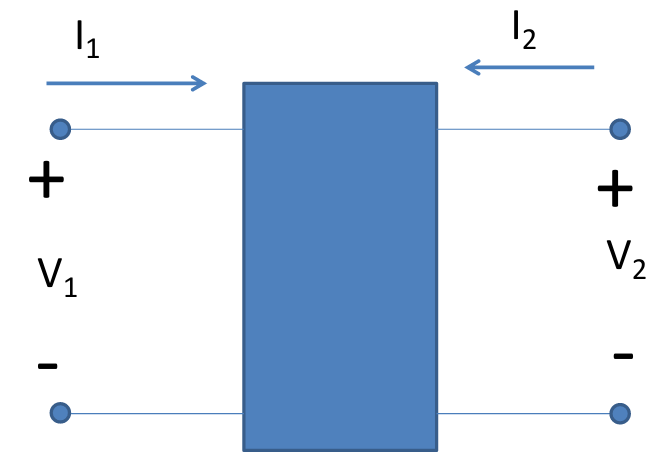
\includegraphics[scale=0.5]{imagens/a7.png} 
			\caption{Corpo rígido realizando movimento plano}
		\end{figure}	
		Os produtos de inércia que envolvem o eixo perpendicular ao plano de referência são nulos (Pxz = Pyz = 0, Px’z’ = Py’z’ = 0). Portanto a quantidade de movimento angular em relação ao centro de massa G é:
		\begin{equation}
			\{H_G\} = \begin{bmatrix}
			J_{x'} & -P_{x'y'} &0\\
			-P_{x'y'} & J_{y'} & 0\\
			0 & 0 & J_{z'}
			\end{bmatrix} = \begin{bmatrix}
			0\\0\\ \omega
			\end{bmatrix} = \begin{bmatrix}
			0\\0\\J_{z'}\omega
			\end{bmatrix}
		\end{equation}
		Ou,
		\begin{equation}
			\vec{H}_G = J_{z'}\omega \vec{k}
		\end{equation}
		Equações de Euler:
		\begin{equation}
			\sum\vec{F} = m\vec{a}_G
		\end{equation}
		\begin{equation}
			\sum\vec{M}_G = J_{z'}\alpha \vec{k}
		\end{equation}

	\subsubsection{Equações de Newton-Euler para o movimento plano de rotação baricêntrica}
		Entendemos por rotação baricêntrica o caso de movimento plano em que, devido à existência de restrições cinemáticas, o corpo rígido gira em torno de um eixo perpendicular ao plano de referência que passa pelo seu centro de massa. 
		\begin{equation}
			\sum\vec{F} = 0
		\end{equation}
		\begin{equation}
			\sum\vec{M}_G = J_{z'}\alpha \vec{k}
		\end{equation}

	\subsubsection{Equações de Newton-Euler para o movimento plano de rotação não baricêntrica}
		A rotação não baricêntrica é o caso de movimento plano em que, devido à existência de restrições cinemáticas, o corpo rígido gira em torno de um eixo perpendicular ao plano de referência que passa por um ponto O não coincidente com seu centro de massa.\\
		
		As equações de Newton Euler assumem as seguintes formas:
		\begin{equation}
			\sum\vec{F} = m\alpha\vec{k} \times \vec{OG} - m\omega^2 \vec{OG}
		\end{equation}
		\begin{equation}
			\sum\vec{M}_O = J_z\alpha\vec{k}
		\end{equation}
		De acordo com o Teoremas dos Eixos Paralelos para os momentos de inércia de massa:
		\begin{equation}
			J_z = J_{z'} + m |\vec{OG}|^2
		\end{equation}

	\subsection{Equações de Newton-Euler para corpos rígidos em movimento tridimensional}
	\subsubsection{Equações de Newton-Euler para corpos rígidos em movimento tridimensional de rotação em torno de um eixo fixo}
		\begin{figure}[h]
			\center
			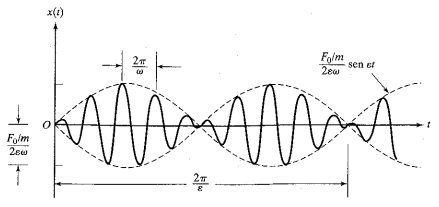
\includegraphics[scale=0.5]{imagens/a8.png} 
			\caption{Corpo rígido desenvolvendo movimento tridimensional de rotação em torno de um eixo fixo}
		\end{figure}
		\begin{equation}
			\{H_O\} = [J_{OXYZ}]\{\omega \}
		\end{equation}
		Pelo teorema dos eixos paralelos:
		\begin{equation}
			[J_{OXYZ}] = \begin{bmatrix}
			J_{x'} & -P_{x'y'} & -P_{x'z'}\\
			-P_{x'y'} & J_{y'} & -P_{y'z'}\\
			-p_{x'z'} & -P_{y'z'} & J_{z'}
			\end{bmatrix} + m\begin{bmatrix}
			 Y_G^2 + Z^2_G & -X_GY_G & -X_GZ_G\\
			 -X_GY_G & X^2_G+Z^2_G & -Y_GZ_G\\
			 -X_GZ_G & -Y_GZ_G & X^2_G + Y_G^2
			\end{bmatrix}
		\end{equation}
		Ao derivar $\{H_O\}$, temos a seguinte relação
		\begin{equation}
			\boxed{
			\sum \{M_O\} = [J_{OX_1Y_1Z_1}]\underbrace{\frac{d\{\omega_1 \}}{dt}|_{Ox1y1z1}}_{\text{a. angular total do corpo rigido}} + \underbrace{\{\omega_2 \}}_{\text{v. do sistema movel}} \times \{H_O\}
			}
		\end{equation}
		E para as forças
		\begin{equation}
			\sum F = ma_G
		\end{equation}

		\subsubsection{Introdução do movimento de giroscópios}
		Um giroscópio consiste, essencialmente, de um corpo com simetria de revolução (axissimetria), que pode girar livremente em torno de um ou mais de seus eixos.\\
		
		Os ângulos $\phi , \theta , \psi$ são conhecidos como ângulos de Euler e suas taxas de variação temporais  $\dot{\phi} , \dot{\theta} , \dot{\psi}$ são, respectivamente, os movimentos de \textit{precessão, nutação e rotação própria}.
		\begin{figure}[h]
			\center
			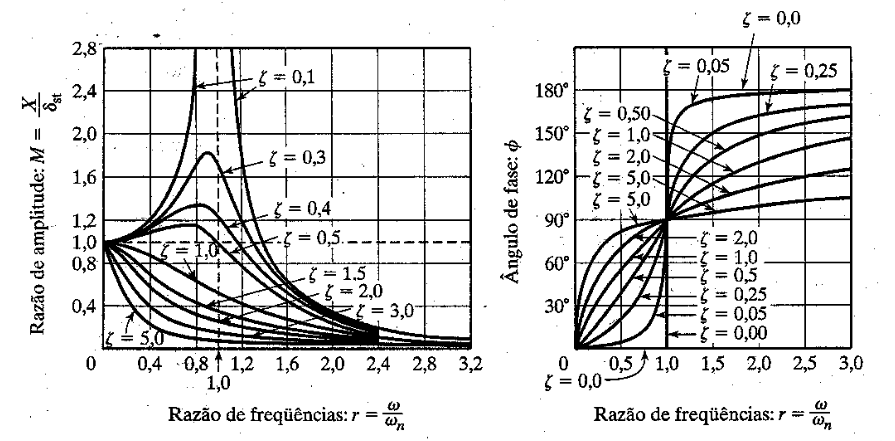
\includegraphics[scale=0.5]{imagens/a9.png} 
			\caption{Ângulos de Euler para o giroscópio}
		\end{figure}
		
		Sendo $z_1$ o eixo em relação ao qual o disco apresenta simetria de revolução, o tensor de inércia do disco em relação ao sistema de referência $G_{x_1y_1z_1}$ tem a forma:
		\begin{equation}
			[J_{G_{x_1y_1z_1}}] = \begin{bmatrix}
			J & 0 & 0\\
			0 & J & 0\\
			0 & 0 & J_p
			\end{bmatrix}
		\end{equation}

		As equações de newton euler ficam:
		\begin{figure}[h]
			\center
			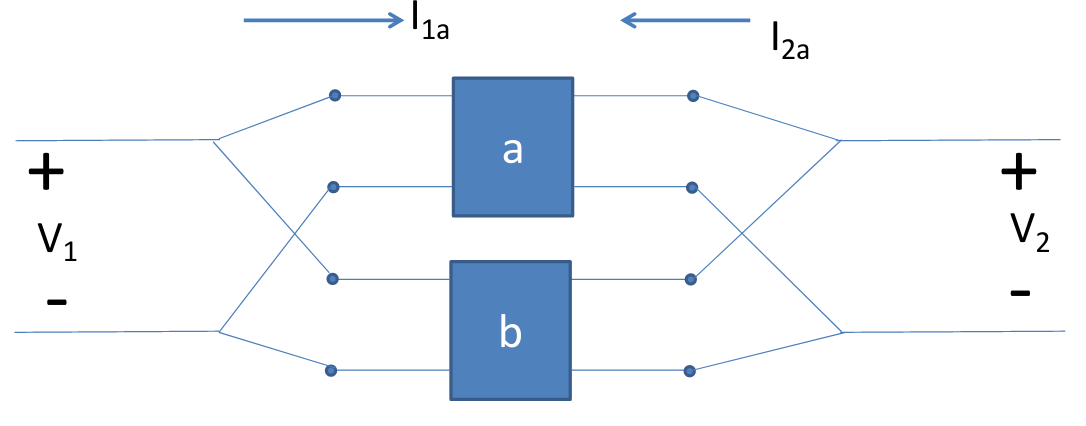
\includegraphics[scale=0.7]{imagens/a10.png} 
			\caption{Equações de Newton-Euler para o giroscópio}
		\end{figure}

		Na \textbf{precessão estacionária de giroscópios} o ângulo $\theta$ é mantido fixo e as taxas de precessão $\phi$ e de rotação própria $\psi$ são constantes, temos:
		 \begin{figure}[h]
			\center
			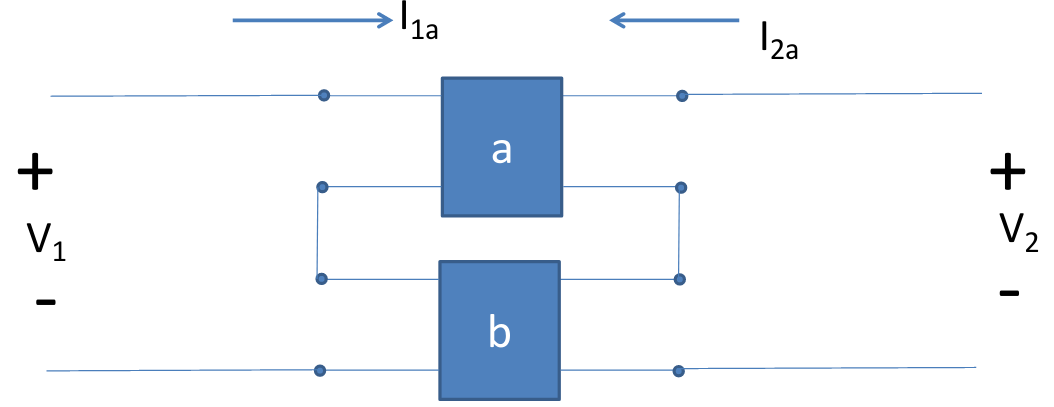
\includegraphics[scale=0.7]{imagens/a11.png} 
			\caption{Precessão estacionária}
		\end{figure}

		\subsubsection{Princípio do Impulso-Quantidade de Movimento para os corpos rígidos. Conservação das quantidades de movimento linear e angular}
		Para um corpo rígido temos:
		\begin{equation}
			\vec{L}(t_2) = \vec{L}(t_1) + \int^{t_2}_{t_1} \sum \vec{F}dt
		\end{equation}
		\begin{equation}
			\vec{H_O}(t_2) = \vec{H_O}(t_1) + \int^{t_2}_{t_1} \sum \vec{M_O}dt
		\end{equation}
		Ou, para o CG
		\begin{equation}
			\vec{H_G}(t_2) = \vec{H_G}(t_1) + \int^{t_2}_{t_1} \sum \vec{M_G}dt
		\end{equation}
		Com $\{H_G(t)\} = [J_{G_{x'y'z'}}]\{\omega (t)\}$\\
		
		\textbf{Movimento plano de rotação não baricêntrica}\\
		\begin{equation}
			J_Z\omega_1 + \int^{t_2}_{t_1} \sum M_Odt = J_Z \omega_2
		\end{equation}

		\newpage
		\subsubsection{Princípio do Impulso-Quantidade de Movimento para corpos rígidos em movimento de rotação em torno de um eixo fixo}
		\begin{figure}[h]
			\center
			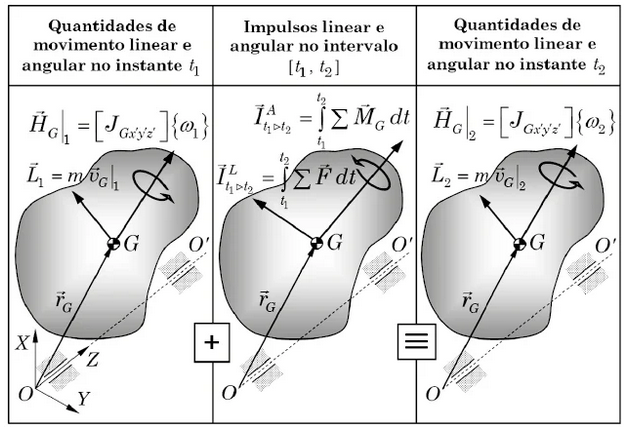
\includegraphics[scale=0.7]{imagens/b1.png} 
			\caption{Movimento de rotação em torno de um eixo fixo}
		\end{figure}
		\begin{equation}
			\vec{H_O}|_1 + \int^{t_2}_{t_1} \sum \vec{M_O} dt = \vec{H_O}|_2
		\end{equation}	
		Com,
		\begin{equation}
			\{\vec{H_O}|_1\} = [J_{OXYZ}]\{\omega_1\}
		\end{equation}
		\begin{equation}
			\{\vec{H_O}|_2\} = [J_{OXYZ}]\{\omega_2\}
		\end{equation}

		
	\subsection{Princípio do Trabalho-Energia Cinética e Princípio da Conservação da Energia Mecânica para os corpos rígidos}
	O trabalho realizado por um momento é dado por:
	\begin{equation}
		W_{1-2}^T = \int^{\theta_2}_{\theta_1} T d\theta
	\end{equation}

	O \textbf{Princípio da Conservação da Energia Mecânica} é expresso sob a forma:
	\begin{equation}
		T_1 + W_{1-2} = T_2
	\end{equation}
	Onde $W_{1-2}$ é a soma dos trabalhos das \textit{forças} e \textit{momentos}.\\
	
	Já o \textbf{Princípio da Conservação da Energia Mecânica} para os corpos rígidos é dada por:
	\begin{equation}
		T_1 + V_1 = T_2 + V_2
	\end{equation}

	\subsubsection{Energia Cinética em Corpos Rígidos}
	A energia cinética em um corpo rígido é dada por:
	\begin{equation}
		T = \frac{1}{2}	m\{v_G\}^T\{v_G\} + \frac{1}{2}\{\omega \}^T[J_{G_{x'y'z'}}]\{\omega \}
	\end{equation}

\section{Momentos de inércia de alguns sólidos de geometria simples}
	\begin{figure}[h]
		\center
		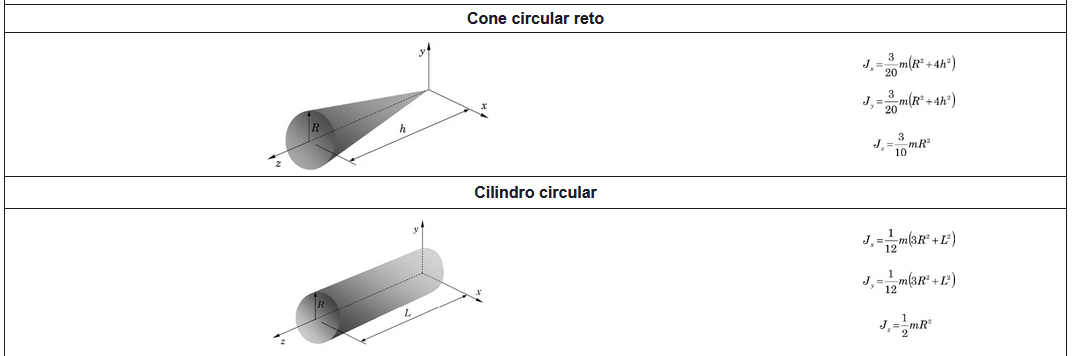
\includegraphics[scale=0.7]{imagens/b2.png} 
	\end{figure}
	\begin{figure}[h]
		\center
		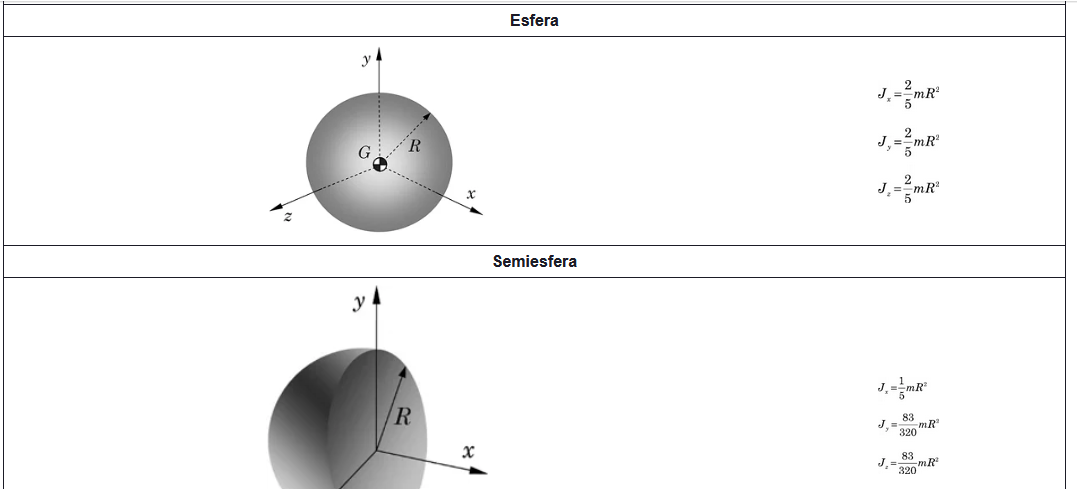
\includegraphics[scale=0.7]{imagens/b3.png} 
	\end{figure}
	\begin{figure}[h]
		\center
		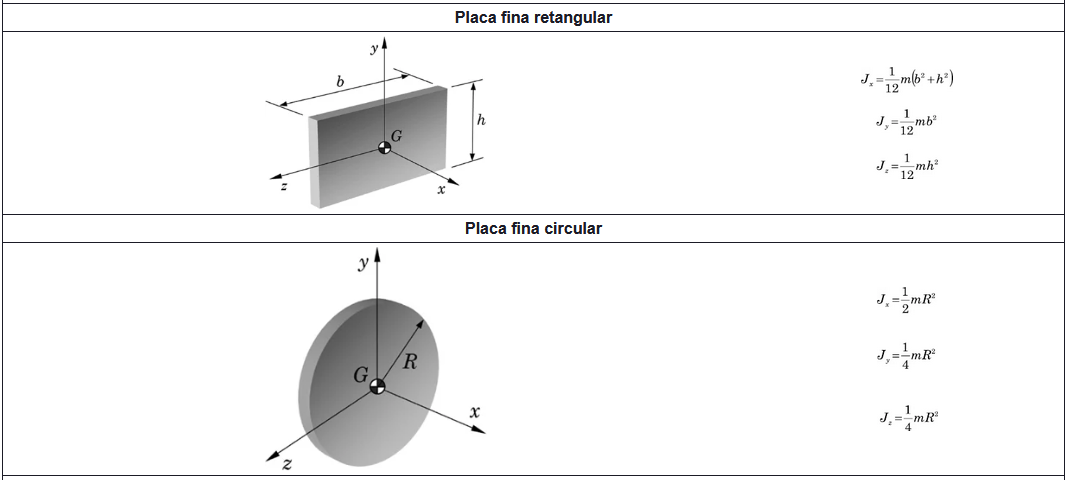
\includegraphics[scale=0.7]{imagens/b4.png} 
	\end{figure}
	\begin{figure}[h]
		\center
		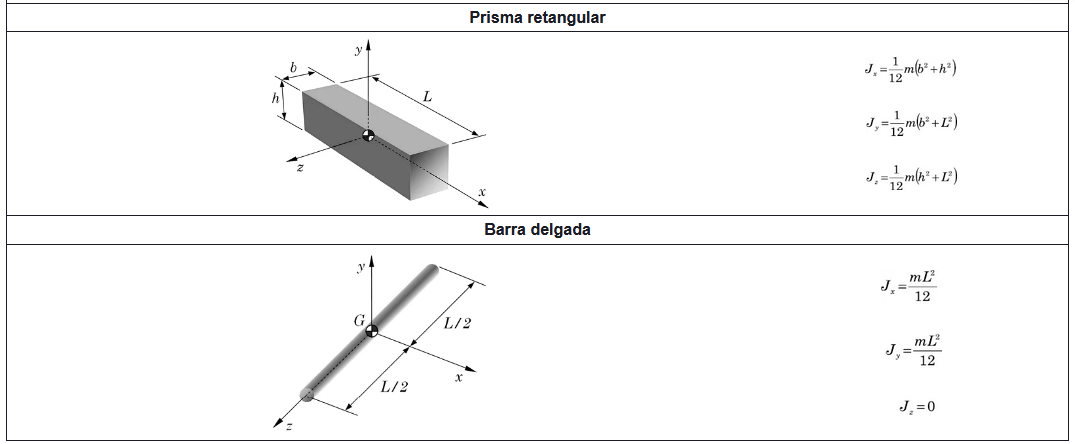
\includegraphics[scale=0.7]{imagens/b5.png} 
	\end{figure}































































































































































































































































\end{document}
